\section{System Architecture}
\label{sec:architecture}

The FlashBoost architecture is a homogeneous cluster of host servers coupled
with a FlashBoost storage device. Each FlashBoost storage device is plugged into
the host server via a PCIe link, and it consists of flash storage, an in-storage
processing engine, 8 high-speed network interfaces and on-board DRAM. The host
servers are networked together using Ethernet or other general-purpose
networking fabric. The host server can access the FlashBoost storage device via
a host interface implemented over PCIe. It can either directly communicate with
the flash interface, to treat is as a raw storage device, or with the in-store
processor to perform computation on the data.

The in-store processing engine has access to four major services: The flash
controller, network controller, host interface and the DRAM Buffer.
Figure~\ref{fig:ispservice} shows the four services. 


\begin{figure}[h]
	\begin{center}
	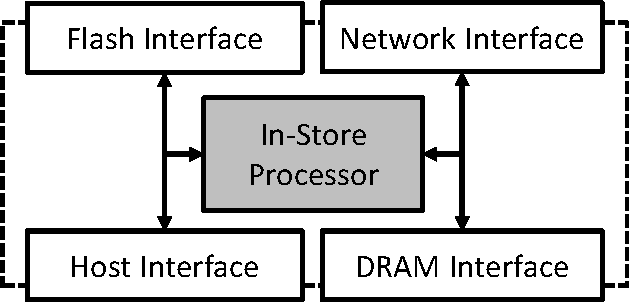
\includegraphics[width=0.3\paperwidth]{figures/isp-service-crop.pdf}
	\caption{Services Provided to In-Store Processor}
	\label{fig:ispservice}
	\end{center}
\end{figure}

In our implementation of FlashBoost, we have used a Field Programmable Gate
Array (FPGA) to implement the in-store processor and also the flash, host and
network controllers. However, the FlashBoost Architecture should not be limited
to an FPGA-based implementation.  Development of FlashBoost was done in the
high-level hardware description language Bluespec. As a result, all services
expose a high-level language interface using latency-insensitive FIFOs for
communication. This makes the services intuitive to use, and flexible to be used
easily with many in-storage processing engines.

\begin{figure*}[ht]
	\begin{center}
	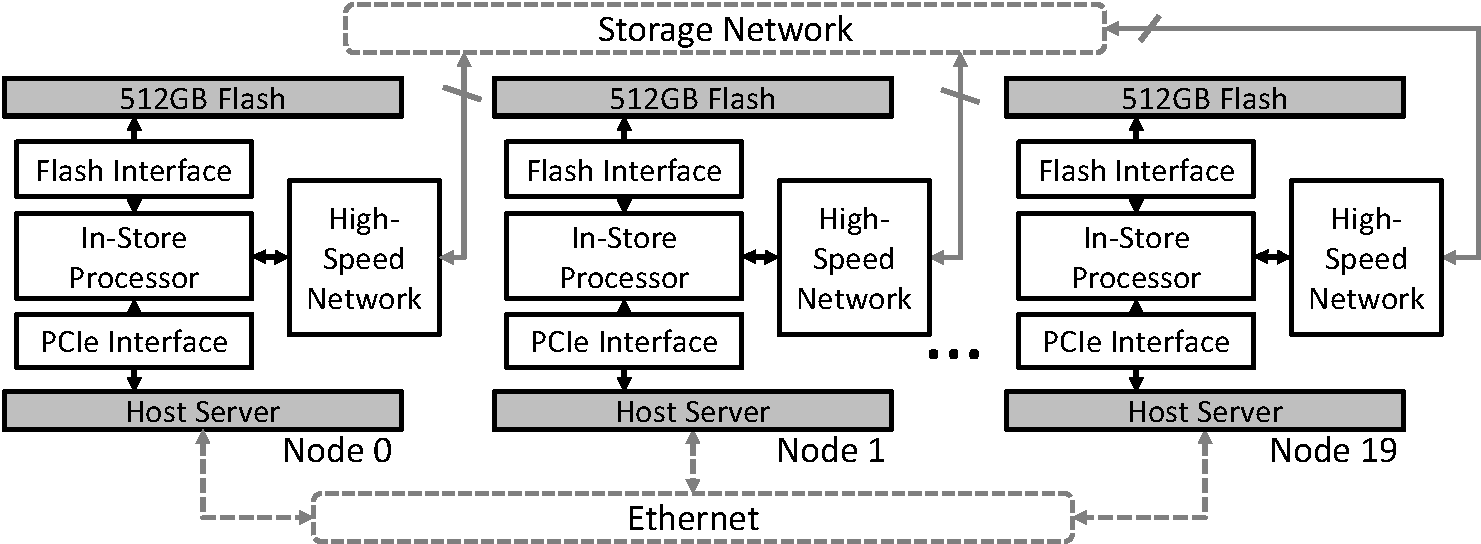
\includegraphics[width=0.8\paperwidth]{figures/architecture.pdf}
	\caption{FlashBoost Architecture}
	\label{fig:architecture}
	\end{center}
\end{figure*}

\subsection{Flash Interface}

Access to flash storage is provided by the flash controller via a
fast, low-level and error-free interface with minimal bandwidth and
latency overhead. This interface exposes the internal memory organization of
the flash device, namely the buses/channels, chips, blocks and pages.
The interface is designed to stream data in
and out of the flash chips as fast as possible without concern for
flash management. Garbage collection, bad block management and
wear-leveling functionalities are handled by the flash-aware file system
in the host kernel (discussed in Section~\ref{sec:software}). The key advantage of such
a low-level interface is that in-store processors have direct access to
the data in a streaming fashion with minimal buffering and insignificant
latency overhead. 

The raw flash interface, in hardware, is defined below:

%[captionpos=b, caption={Flash Controller Interface}, label={lst:hwifc}]
\begin{lstlisting}
interface FlashIfc;       
  method sendCmd (FlashOp op, Bit#(4) bus,
                  Bit#(3) chip, Bit#(16) block, 
                  Bit#(8) page, Bit#(8) tag);        
  method writeWord (Bit#(128) data, Bit#(8) tag);
  method Tuple2#(Bit#(128), Bit#(8)) readWord (); 
  method Bit#(8) writeDataReq ();
  method Tuple2#(Bit#(8), StatusT) ackStatus ();
endinterface 
\end{lstlisting}

To access the flash, the user issues a flash command
(\textit{sendCmd} method) with the operation, the address and
a free tag. For writes, the user awaits for a write data request from
the controller scheduler (\textit{writeDataReq} method), and then sends
the write data corresponding to that request in 128-bit bursts
(\textit{writeWord} method). An acknowledgement is received when the
operation completes (\textit{ackStatus} method). For read operations,
data will return in 128-bit bursts along with the command tag that the
burst corresponds to. We emphasize that for maximum performance, the
controller sends these data bursts \textbf{out of order} with respect to
the issued request and \textbf{interleaved} with other read requests.
Thus completion buffers may be required on the user side. Furthermore,
we note that to saturate the bandwidth of the flash device, multiple
commands must be in-flight at the same time, since flash operations
have latencies of tens to thousands of microseconds. 

In our architecture, multiple users may need shared access to the
flash controller interface. For example, a particular flash controller may
be accessed by local in-store processors, local host software over PCIe
DMA, or remote in-store processors. Thus, we include as part of the
platform, an interface multiplexer that converts one flash interface
into a parametrizable number of additional interfaces. 

%TODO: give a name to this module?
To ease development of hardware accelerators (i.e. in-store processors),
we also provide a parametrizable module that converts a flash interface
into multiple simple in-order request/response interfaces
(Figure~\ref{?}). We allow the user to adjust the interface width, the
command queue depth and number of interfaces of the converter.
Internally, the converter renames tags and uses completion buffers to
order data. This design easily permits multiple accelerators to be
attached to the flash device, taking advantage of flash parallelism. 


\begin{figure}[h]
	\begin{center}
	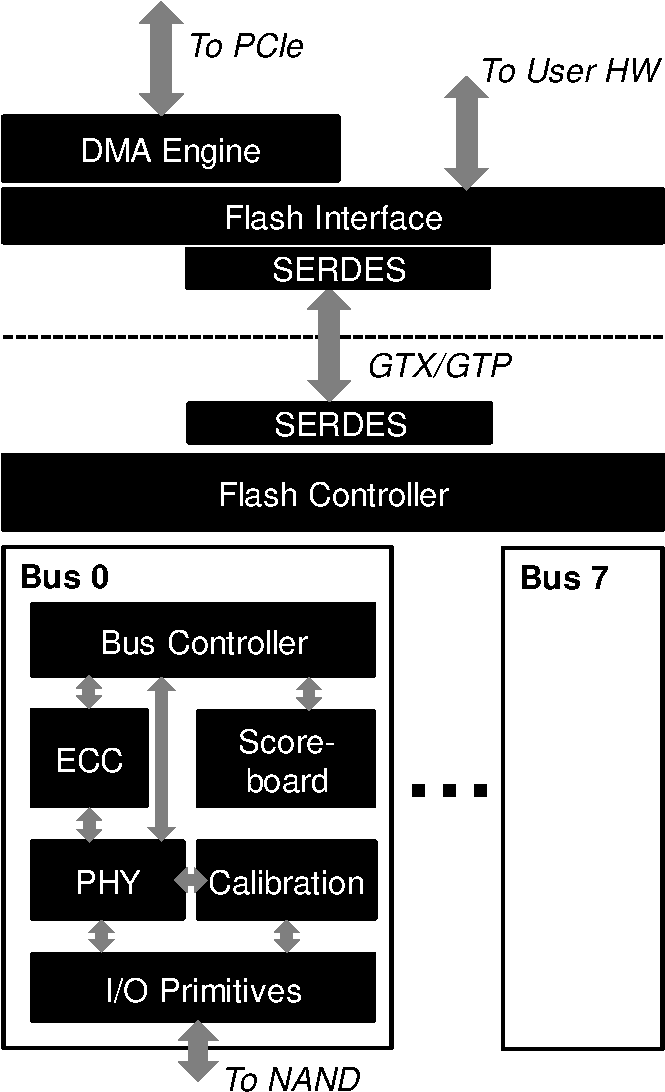
\includegraphics[scale=0.4]{figures/top-arch-crop.pdf}
	\caption{Flash Interface}
	\label{fig:flashinterface}
	\end{center}
\end{figure}

\subsection{Integrated Storage Network}


FlashBoost provides a low-latency high-bandwidth network infrastructure across
all FlashBoost storage devices in the cluster.  FlashBoost storage devices are
linked among themselves via high-performance serial links that are separate from
the host server network. For data traffic between the storage devices, the
integrated network ports removes the overhead of going through software to
access a separate network interface.

Each storage device has multiple network ports, and
acts both as a network switch as well as a network client. The storage network
functionality such as routing, flow control and virtual channels while
maintaining high performance an extremely low latency.

\subsubsection{Network Endpoint}

The FlashBoost network infrastructure exposes virtual channel semantics to the
in-storage processor by providing it with a vector of endpoints. Each endpoint
exposes two interfaces, \texttt{send} and \texttt{receive}. An in-storage
processor can send data to a remote node by calling \texttt{send} with a pair of
data and destination node index, or receive data from remote nodes by calling
\texttt{receive}, which returns a pair of data and source node index. These
interfaces provide back pressure, so that each endpoint can be treated like a FIFO
interface across the whole cluster. Such intuitive characteristics of the
network ease in-storage processor development.

\subsubsection{Link Layer}

The link layer manages physical connections between network ports in the storage
nodes. The most important aspect of the link layer is the simple token-based
flow control implementation. This provides back pressure across the link and
assures that no packet will drop if the data rate is higher than what the
network can manage, or if the data is not received from the destination node
quick enough.

\subsubsection{Routing Layer}

The goals of the FlashBoost network infrastructure is to maintain a simple
design while maintaining high bandwidth and low latency, and this requirement
prompted many design choices.

One important aspect of the routing design is that the routing table can have
more than one network port entry per node index. This is because each pair of
nodes can have more than one immediate link connecting between them, and there may be
multiple viable paths between a pair of two remote nodes. In order to make
maximum use of the available bandwidth in such cases, the routing table can have
entries for multiple valid ports for the next hop. In order to ensure in-order
arrival, the endpoint id of the origin endpoint is hashed to deterministically
decide which entry to use in the routing table. In-order arrival is desirable in
a hardware implementation because completion buffers may be expensive. If an
in-storage processing engine wants higher bandwidth for a single bus, it can
break a wide data bus into multiple endpoints and send them over in parallel.
Figure~\ref{fig:networkrouting} shows packet routing in an example network.
The routing table is populated by the software during initialization. And if the
software wants to direct more traffic over a certain link, it can choose to
populate the routing table with more than one instances of the same port.


\begin{figure}[h]
	\begin{center}
	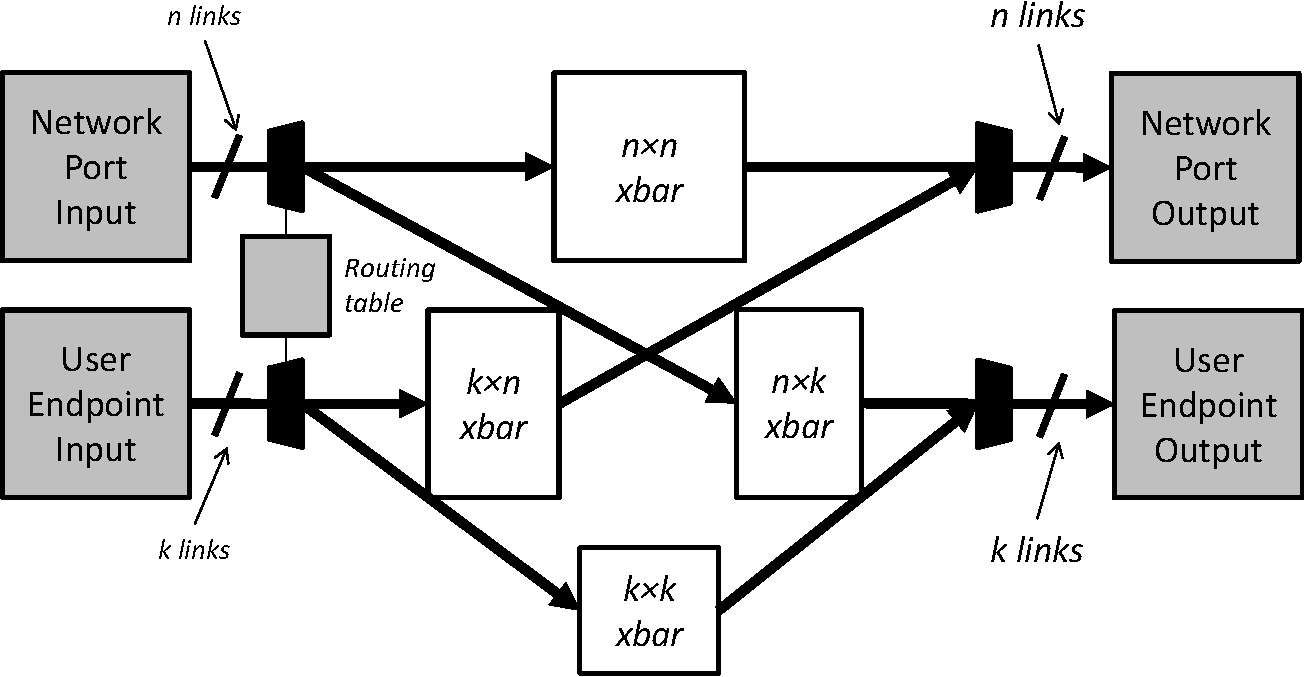
\includegraphics[scale=0.4]{figures/network-routing-crop.pdf}
	\caption{Router Architecture}
	\label{fig:networkinterface}
	\end{center}
\end{figure}

It should be noted that the infrastructure does not assure that the receiving
side will always be able to receive the data being transferred. If a destination
endpoint is unable to receive data at a fast enough rate, it might result in
related parts of the network being blocked. This was an intentional design
choice to build an extremely low-latency network while maintaining low resource
usage. The programmer can choose to use our provided end-to-end flow control
module on top of the network infrastructure to ensure the data source will only
send data that the receiver have space for, but this results higher network
latency as flow control packets frequently needs to be sent to ensure free space
on the receiving end, and also consumes a large amount of memory, which can be
scarce on an embedded system.  On the other hand, if the designer is sure that
the packets will always be consumed, such additional layers can be omitted. 

Figure~\ref{fig:networkinterface} shows the implementation of the router in each
storage node. Each packet can either come from the network port's link layer
interface, or from the user's network endpoint. Each incoming packet's
destination field is compared to the routing table in the router to determine
whether to be forwarded to a remote node via a network port, or to be delivered
to a local endpoint if its destination is the current node. It then goes through
one of the four crossbar switches to be delivered to the correct destination. 
Fairness is implemented using a round-robin priority ordering to ensure maximum
throughput while ensuring no port starves.

\begin{figure}[h]
	\begin{center}
	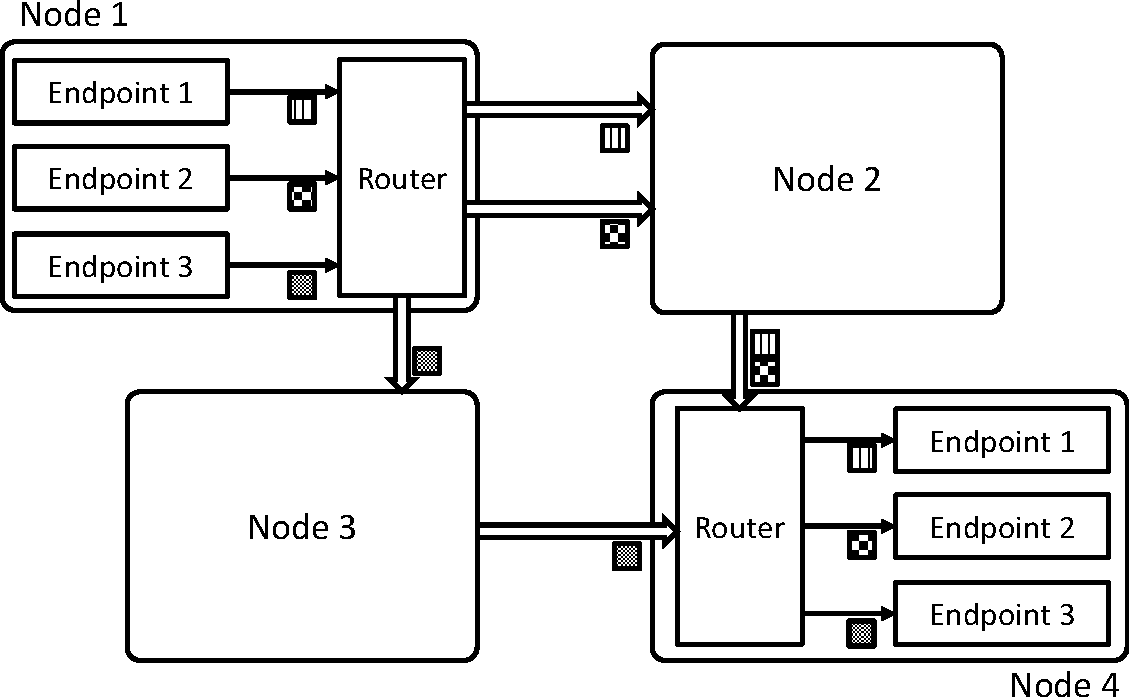
\includegraphics[width=0.4\textwidth]{figures/routing-crop.pdf}
	\caption{Routing Packets Across the Network}
	\label{fig:networkrouting}
	\end{center}
\end{figure}


\subsection{Host Interface}

The in-storage processing core can be accessed from the host server over either
a direct interface that supports RPC and DMA operations, or a file system
abstraction built on top of the direct interface. The file system interface is
described in detail in Section~\ref{sec:software}.

In order to parallelize requests and maintain high performance, the host
interface provides the software with 128 page buffers, each for reads and
writes. When writing a page, the software will request a free write buffer, copy
data to the write buffer, and send a write request over RPC with the
physical address of the destination flash page.
data from that buffer. The buffer will be returned to the free queue when the
hardware has finished reading the data from the buffer. When reading a page, the
software will request a free read buffer, and send a read request over RPC with
the physical address of the source flash page. The software will receive an
interrupt with the buffer index when the hardware has finished writing to
software memory.

Using DMA to write data to the storage device is straightforward to parallelize,
but parallelizing reads is a bit more tricky, due to the characteristics of flash
storage. When writing to storage, the DMA engine on the hardware will read data
from each buffer in order in a contiguous stream. So having enough requests in
the request queue is enough to make maximum use of the host-side link bandwidth.
However, data read from flash chips on multiple buses in parallel can arrive
interleaved at the DMA engine. Because the DMA engine needs to have enough
contiguous data for a DMA burst before issuing a DMA burst, some reordering may
be required at the DMA engine. This becomes even more tricky when the device is
using the integrated network to receive data from remote nodes, where they might
all be coming from different buses. To fix this issue, we provide dual-ported
buffer in hardware providing the semantics of a vector of FIFOs, so that data
for each request can be enqueued into its own FIFO until there is enough data
for a burst.
Figure~\ref{fig:hostinterface} describes the structure of the host
interface.

\begin{figure}[ht!]
	\centering
%	\subfloat[Writing Data to Storage]
%		{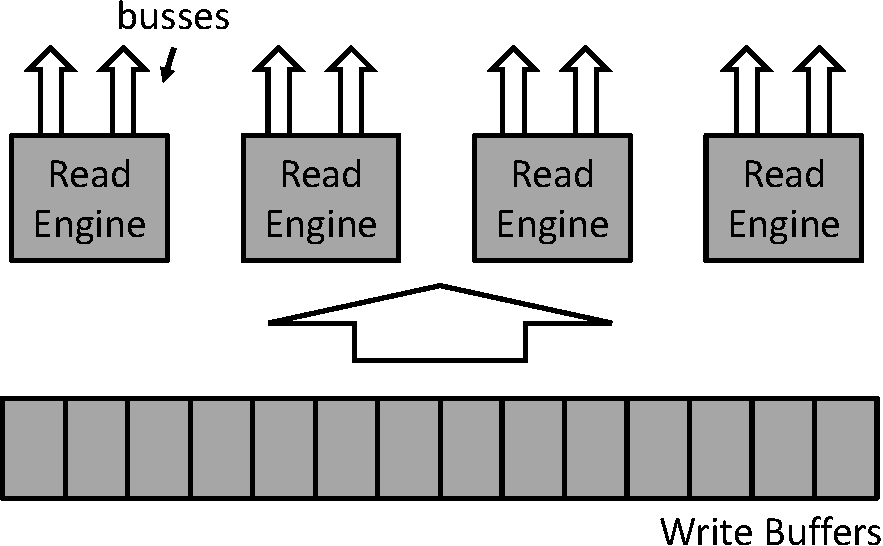
\includegraphics[width=0.23\textwidth]{figures/readinterface-crop.pdf}}
%	\subfloat[Reading Data from Storage]
%		{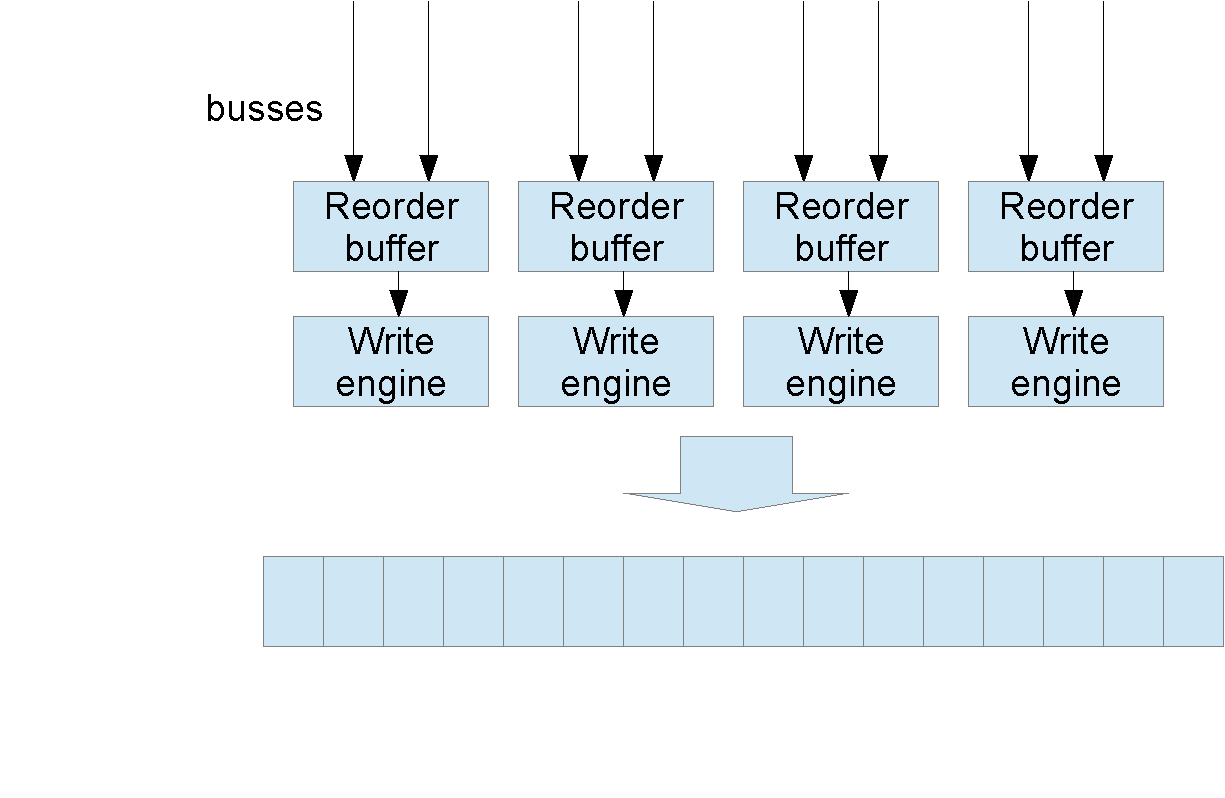
\includegraphics[width=0.23\textwidth]{figures/writeinterface-crop.pdf}}
	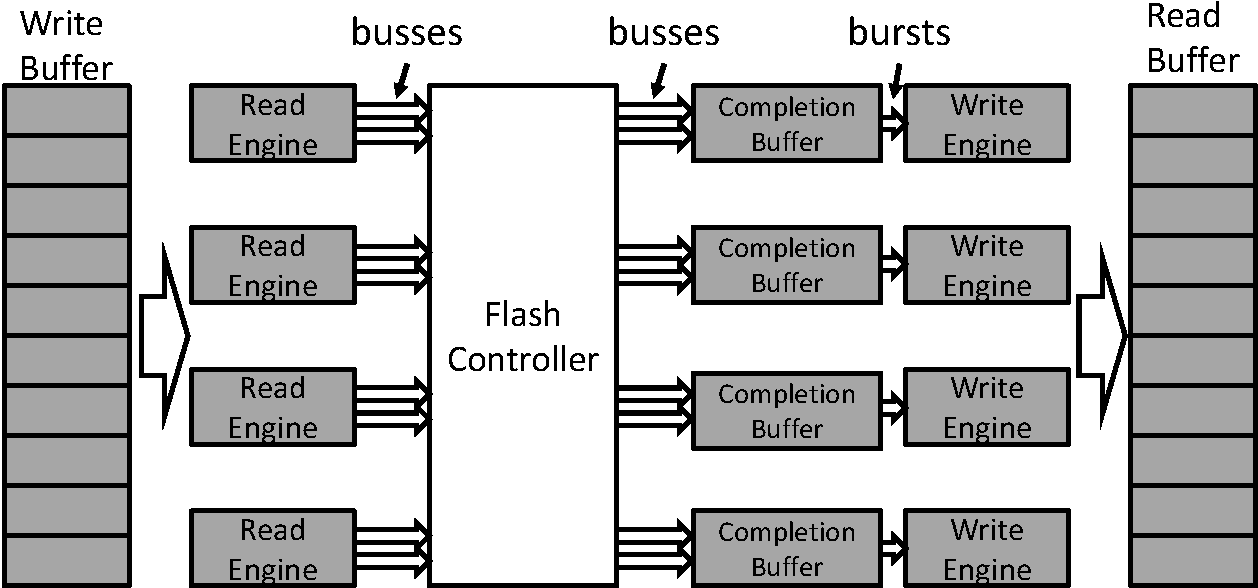
\includegraphics[width=0.4	\textwidth]{figures/hostinterface-crop.pdf}
	\caption{Host-FPGA Interface Over PCIe}
	\label{fig:hostinterface}
\end{figure}

%TODO: \subsubsection{Storage Bridge to Host}
